% MAT670 -- Interlude D (after Lecture 11): min-max, configuration spaces and braids.
% Entirely new material (not in the handwritten notes). Labels prefixed TOP:.

\chapter[Interlude D: Min-max and braids]{Interlude D: Min-max, configuration spaces and braids}
\label{TOP:ch}

\begin{addedblock}
This interlude is new: it is not in the handwritten notes. It takes three threads from
Lectures~7--11 (the deformation theorem of Lecture~9, the max-min distance function and its balanced
contact graphs in Lectures~10--11, and the braid groups of Lecture~7) and follows each one into a
neighbouring field. To keep it readable it is set in black; all of it should be read as added material.
\end{addedblock}

Lectures~8--11 used Morse theory in two ways. For smooth functions, the Morse inequalities count critical
points of \emph{non-degenerate} functions by Betti numbers. For the min-type function
\[
  \rho(u)=\min_{i<j}d(u_i,u_j)\qquad\text{on }\Conf(N,\Sph^2),
\]
we only had a deformation theorem: the topology of $\{\rho\ge\theta\}$ changes only at balanced
configurations. This leaves some natural questions open.
\begin{itemize}
\item The deformation theorem alone already forces critical points to exist, without any
  non-degeneracy. How many, and why?
\item What do the Betti numbers of $\Conf(N,\Sph^2)/\SO(3)$ computed in Lecture~10 say about energies on
  that space, and why are they products like $(1+2t)(1+3t)\cdots$?
\item Lecture~7 defined braid groups as fundamental groups and Lecture~8 found the Weyl chambers of
  $A_{N-1}$ inside $\Conf(N,\R)$. Are these two facts related?
\end{itemize}
The answers lead to \emph{min-max theory} (Section~\ref{TOP:sec:minmax}), to Morse theory on
\emph{configuration spaces of hard particles} (Sections~\ref{TOP:sec:mintype}--\ref{TOP:sec:conf}),
and to \emph{braid and Artin groups} (Section~\ref{TOP:sec:braids}). Section~\ref{TOP:sec:gallery}
collects theorems from these areas.

Throughout, $M$ is a connected smooth manifold with a Riemannian metric and $f\colon M\to\R$ is
smooth. As in Lecture~9, $M^a=f^{-1}(-\infty,a]$. We say that $f$ has \emph{compact sublevel sets} if
every $M^a$ is compact. This holds when $M$ is compact, and also for energies such as
$\sum_{i<j}\abs{u_i-u_j}^{-1}$ on $\Conf(N,\Sph^2)$, which blow up at collisions.

%======================================================================
\section{From Morse theory to min-max}
\label{TOP:sec:minmax}

\subsection{The deformation lemma and the minimax principle}

The proof of Theorem~\ref{L9:thm:diffeo} gives slightly more than its statement. We record the
version we need.

\begin{lemma}[Deformation lemma]\label{TOP:lem:deform}
Let $f$ have compact sublevel sets, let $a<b$ and $\delta>0$, and suppose that $f^{-1}[a-\delta,b+\delta]$
contains no critical point. Then there are diffeomorphisms $\eta_t\colon M\to M$, $0\le t\le1$,
depending smoothly on $t$, with $\eta_0=\mathrm{id}$, $\eta_1(M^b)\subseteq M^a$, and $\eta_t(x)=x$
for all $t$ whenever $f(x)\le a-\delta$ or $f(x)\ge b+\delta$.
\end{lemma}

\begin{proof}
Choose a smooth $\chi\colon\R\to[0,1]$ with $\chi=1$ on $[a,b]$ and support in $(a-\delta,b+\delta)$, and
put
\[
  X=\chi(f)\,\frac{\nabla f}{\abs{\nabla f}^2}.
\]
This is smooth, because $\nabla f\neq0$ on the support of $\chi(f)$, and it vanishes outside the compact set
$f^{-1}[a-\delta,b+\delta]$. By Lemma~\ref{L9:lem:flow} it generates a one-parameter group $\varphi_t$. Along
a flow line, $\frac{d}{dt}f(\varphi_t(x))=df(X)=\chi(f)\in[0,1]$, with value $1$ while $f\in[a,b]$. Set
$\eta_t=\varphi_{-t(b-a)}$. Running the flow backwards for time $b-a$, a point with $f(x)\le b$ either
starts below $a$ and stays there ($f$ is non-increasing), or loses height at unit rate until it reaches
$a$. So $\eta_1(M^b)\subseteq M^a$. Points where $X=0$ are fixed by the flow, which gives the last claim.
\end{proof}

The lemma says that \emph{if there is no critical value near $c$, then everything up to level $c+\varepsilon$
can be pushed below $c-\varepsilon$.} Turning this around produces critical points.

\begin{theorem}[Minimax principle]\label{TOP:thm:minimax}
Let $f$ have compact sublevel sets. Let $Z\subseteq M$ be a set (possibly empty) and let $\mathcal F$ be a
family of non-empty subsets of $M$ such that $\eta_1(A)\in\mathcal F$ whenever $A\in\mathcal F$ and
$(\eta_t)$ is an isotopy of diffeomorphisms of $M$ fixing $Z$ pointwise. Put
\[
  c=\inf_{A\in\mathcal F}\ \sup_{x\in A}f(x).
\]
If $c<\infty$ and $\sup_Zf<c$, then $c$ is a critical value of $f$.
\end{theorem}

\begin{proof}
Since $f$ attains its minimum, $c>-\infty$. The critical points in $f^{-1}[c-1,c+1]$ form a compact
set, so their values form a compact set. If $c$ is not critical, there is therefore an $\varepsilon>0$ such
that $[c-3\varepsilon,c+3\varepsilon]$ contains no critical value; shrinking $\varepsilon$, we may also assume
$\sup_Zf<c-2\varepsilon$. Apply Lemma~\ref{TOP:lem:deform} with $a=c-\varepsilon$, $b=c+\varepsilon$,
$\delta=\varepsilon$. The isotopy fixes $\{f\le c-2\varepsilon\}\supseteq Z$. Pick $A\in\mathcal F$ with
$\sup_Af\le c+\varepsilon$. Then $\eta_1(A)\in\mathcal F$ and $\eta_1(A)\subseteq M^{c-\varepsilon}$, so
$\sup_{\eta_1(A)}f\le c-\varepsilon<c$, contradicting the definition of $c$.
\end{proof}

\begin{example}\label{TOP:ex:families}\leavevmode
\begin{enumerate}[nosep]
\item $\mathcal F=\{\{x\}:x\in M\}$ gives $c=\min f$. If $M$ is compact, $\mathcal F=\{M\}$ gives $c=\max f$.
\item \emph{Homology classes.} For $0\neq\alpha\in H_k(M)$ let $\mathcal F_\alpha$ be the family of compact
  $A\subseteq M$ such that $\alpha$ lies in the image of $H_k(A)\to H_k(M)$. A diffeomorphism isotopic to
  the identity acts trivially on homology, so $\mathcal F_\alpha$ is invariant. The critical value
  $c_\alpha$ is ``the lowest level at which $\alpha$ can be realized''. For the height function on the
  torus of Example~\ref{L07:ex:torus}, the classes in $H_1$ give the two saddle values $f(q)$ and $f(r)$.
\item \emph{Mountain pass.} For $p,q\in M$, take $Z=\{p,q\}$ and $\mathcal F=\{\gamma([0,1]):\gamma
  \text{ a path from }p\text{ to }q\}$.
\end{enumerate}
\end{example}

\begin{corollary}[Mountain pass]\label{TOP:cor:mp}
Let $f$ have compact sublevel sets and let $p\neq q$ be strict local minima of $f$. Then $f$ has a third
critical point, at the level
\[
  c=\inf_{\gamma\colon p\leadsto q}\ \max_{t\in[0,1]}f(\gamma(t))\ >\ \max\big(f(p),f(q)\big).
\]
\end{corollary}

\begin{proof}
Say $f(p)\le f(q)$. Since $q$ is a strict local minimum, a small geodesic sphere $S$ around $q$ (not
containing $p$ inside) satisfies $\min_Sf>f(q)$. Every path from $p$ to $q$ crosses $S$, so
$c\ge\min_Sf>f(q)\ge f(p)$. Also $c<\infty$ because $M$ is connected. Theorem~\ref{TOP:thm:minimax}
with Example~\ref{TOP:ex:families}(3) applies.
\end{proof}

\begin{figure}[ht]
\centering
\begin{tikzpicture}[scale=1.15]
  \draw[gray!70] plot[domain=0:360,samples=120,smooth] ({2.6*cos(\x)/(1+sin(\x)^2)},{2.6*sin(\x)*cos(\x)/(1+sin(\x)^2)});
  \draw[gray!50] (-1.55,0) ellipse (0.55 and 0.3); \draw[gray!50] (1.55,0) ellipse (0.55 and 0.3);
  \draw[gray!50] (-1.55,0) ellipse (0.95 and 0.5); \draw[gray!50] (1.55,0) ellipse (0.95 and 0.5);
  \draw[gray!50] (0,0) ellipse (3.2 and 1.25);
  \fill (-1.55,0) circle (1.5pt) node[below=2pt,font=\small] {$p$};
  \fill (1.55,0) circle (1.5pt) node[below=2pt,font=\small] {$q$};
  \draw[addcol,very thick] (-1.55,0) .. controls (-0.8,0.25) and (-0.3,0) .. (0,0) .. controls (0.3,0) and (0.8,-0.25) .. (1.55,0);
  \fill[flagcol] (0,0) circle (1.8pt) node[above=3pt,font=\small,flagcol] {$s$};
  \draw[thick,dashed] (-1.55,0) .. controls (-1.4,1.3) and (1.4,1.3) .. (1.55,0);
  \fill (0,0.98) circle (1.3pt) node[above,font=\scriptsize] {$\max f\circ\gamma$};
  \node[font=\scriptsize,gray] at (2.85,1.15) {level sets of $f$};
  % profile
  \begin{scope}[xshift=5.2cm,yshift=-0.6cm,scale=0.9]
    \draw[->] (0,0)--(2.9,0) node[right,font=\scriptsize]{$t$};
    \draw[->] (0,0)--(0,2.1) node[above,font=\scriptsize]{$f(\gamma(t))$};
    \draw[addcol,very thick] (0.1,0.3) .. controls (0.7,0.4) and (1.0,1.1) .. (1.4,1.1) .. controls (1.8,1.1) and (2.1,0.55) .. (2.7,0.5);
    \draw[thick,dashed] (0.1,0.3) .. controls (0.6,1.9) and (2.2,1.9) .. (2.7,0.5);
    \draw[dotted] (0,1.1)--(1.4,1.1); \node[left,font=\scriptsize] at (0,1.1) {$c$};
  \end{scope}
\end{tikzpicture}
\caption{The mountain pass. Every path from $p$ to $q$ has a highest point; the dashed path climbs
higher than necessary. The minimax level $c$ is attained by paths through the saddle $s$, where the
level set through $s$ is a figure eight.}
\label{TOP:fig:mp}
\end{figure}

\subsection{Lusternik--Schnirelmann category}

The minimax principle gives one critical value per invariant family. To get many critical points we need
many families, and a way to tell them apart. Lusternik and Schnirelmann (around 1930) measured the
families by how hard it is to contract them.

\begin{definition}\label{TOP:def:cat}
For $A\subseteq M$, the \emph{category of $A$ in $M$}, $\operatorname{cat}_M(A)$, is the least $m$ such that
$A\subseteq U_1\cup\dots\cup U_m$ with each $U_i$ open in $M$ and each inclusion $U_i\hookrightarrow M$
homotopic to a constant map. The \emph{Lusternik--Schnirelmann category} of $M$ is
$\operatorname{cat}(M)=\operatorname{cat}_M(M)$.
\end{definition}

So $\operatorname{cat}(\text{point})=1$ and $\operatorname{cat}(\Sph^n)=2$ (two hemispheres). This is the
unnormalized convention; many papers subtract $1$. The following properties are immediate.
Category is monotone in $A$ and subadditive, $\operatorname{cat}_M(A\cup B)\le\operatorname{cat}_M(A)+
\operatorname{cat}_M(B)$. A homeomorphism of $M$ homotopic to the identity preserves it. A finite set has
category $1$: a union of small disjoint balls can be contracted inside the connected manifold $M$.

\begin{theorem}[Cup-length bound]\label{TOP:thm:cuplength}
If there are classes $u_1,\dots,u_k\in H^*(M)$ of positive degree (any coefficients) with
$u_1\smile\dots\smile u_k\neq0$, then $\operatorname{cat}(M)\ge k+1$.
\end{theorem}

\begin{proof}
Suppose $M=U_1\cup\dots\cup U_k$ with each $U_i\hookrightarrow M$ null-homotopic. Then the restriction
of $u_i$ to $U_i$ factors through the cohomology of a point, which vanishes in positive degree, so
$u_i|_{U_i}=0$. By the long exact sequence of the pair $(M,U_i)$, $u_i$ is the image of some
$\tilde u_i\in H^*(M,U_i)$. The relative cup product (defined for open sets) gives
\[
  \tilde u_1\smile\dots\smile\tilde u_k\in H^*(M,U_1\cup\dots\cup U_k)=H^*(M,M)=0,
\]
and it maps to $u_1\smile\dots\smile u_k$. Hence the product is $0$, a contradiction.
\end{proof}

To count critical points we also need a version of the deformation lemma that is allowed to stop near the
critical points at level $c$.

\begin{lemma}[Deformation with a hole]\label{TOP:lem:hole}
Let $f$ have compact sublevel sets, let $c\in\R$, let $K_c$ be the (compact) set of critical points
with value $c$, and let $U\supseteq K_c$ be open. Then there are $\varepsilon>0$ and a diffeomorphism
$\eta$ of $M$, isotopic to the identity, with $\eta\big(M^{c+\varepsilon}\setminus U\big)\subseteq M^{c-\varepsilon}$.
\end{lemma}

\begin{proof}
Choose open sets $K_c\subseteq V\subseteq\overline V\subseteq U_1\subseteq\overline U_1\subseteq U$ with
$\overline U_1$ compact.

\emph{Step 1: the gradient is bounded below away from $V$ near level $c$.} There are $\varepsilon_0,\sigma>0$
with $\abs{\nabla f}\ge\sigma$ on $f^{-1}[c-\varepsilon_0,c+\varepsilon_0]\setminus V$. Otherwise there are
$x_n\notin V$ with $f(x_n)\to c$ and $\nabla f(x_n)\to0$. They lie in the compact set
$f^{-1}[c-1,c+1]$, so a subsequence converges to some $x\notin V$ with $\nabla f(x)=0$ and $f(x)=c$. Then
$x\in K_c\subseteq V$, a contradiction.

\emph{Step 2: the vector field.} Let $\psi\colon M\to[0,1]$ be smooth with $\psi=0$ on $V$ and $\psi=1$
outside $U_1$, and let $\chi$ be a cutoff with $\chi=1$ on $[c-\varepsilon,c+\varepsilon]$ and support in
$(c-\varepsilon_0,c+\varepsilon_0)$, for an $\varepsilon\le\varepsilon_0/2$ fixed below. Put
$X=\chi(f)\psi\nabla f/\abs{\nabla f}^2$. By Step~1 it is smooth, compactly supported, and
$\abs X\le1/\sigma$. Along its backward flow $f$ is non-increasing, and
$\frac{d}{dt}f=-\chi(f)\psi$.

\emph{Step 3: flow lines from outside $U$ do not reach $U_1$ in time $2\varepsilon$.} Let
$d=\dist(M\setminus U,\overline U_1)>0$. A flow line has speed at most $1/\sigma$, so in time $T$ it travels
at most $T/\sigma$. Choose $\varepsilon$ with $2\varepsilon<d\sigma$. A flow line starting at
$x\notin U$ then stays outside $U_1$, where $\psi=1$, for $0\le t\le2\varepsilon$. If moreover $f(x)\le
c+\varepsilon$, then $f$ drops at unit rate while it lies in $[c-\varepsilon,c+\varepsilon]$, so after time
$2\varepsilon$ we have $f\le c-\varepsilon$. Take $\eta$ to be the backward flow for time $2\varepsilon$.
\end{proof}

\begin{theorem}[Lusternik--Schnirelmann]\label{TOP:thm:LS}
Every smooth function on a compact connected manifold $M$ has at least $\operatorname{cat}(M)$ critical
points.
\end{theorem}

\begin{proof}
Let $m=\operatorname{cat}(M)$ and, for $1\le k\le m$, let $\mathcal F_k$ be the family of closed
$A\subseteq M$ with $\operatorname{cat}_M(A)\ge k$. These families are invariant under diffeomorphisms
isotopic to the identity and nested, $\mathcal F_1\supseteq\dots\supseteq\mathcal F_m\ni M$. So the values
$c_k=\inf_{A\in\mathcal F_k}\max_Af$ satisfy $c_1\le c_2\le\dots\le c_m\le\max f$, and each is critical by
Theorem~\ref{TOP:thm:minimax}. If they are distinct we have $m$ critical points. Suppose instead that
$c_k=c_{k+1}=c$. We claim that $K_c$ is infinite. If not, let $U$ be a union of small disjoint balls around
the points of $K_c$, so that $\operatorname{cat}_M(\overline U)=1$. Take $\varepsilon,\eta$ from
Lemma~\ref{TOP:lem:hole} and $A\in\mathcal F_{k+1}$ with $\max_Af\le c+\varepsilon$. The closed set $B=A\setminus
U$ has $\operatorname{cat}_M(B)\ge\operatorname{cat}_M(A)-\operatorname{cat}_M(\overline U)\ge k$, so
$\eta(B)\in\mathcal F_k$. But $\eta(B)\subseteq M^{c-\varepsilon}$, which gives $c_k\le c-\varepsilon$, a
contradiction.
\end{proof}

The argument also shows that if two of the minimax values coincide, then the critical set at that level
is not just infinite but has category at least $2$ in $M$.

\begin{example}[Three critical points on the torus]\label{TOP:ex:torus}
On $\T^2=\R^2/\Z^2$ the de Rham classes $a=[dx]$ and $b=[dy]$ in $H^1(\T^2;\R)$ have
$a\smile b=[dx\wedge dy]\neq0$. By Theorem~\ref{TOP:thm:cuplength}, $\operatorname{cat}(\T^2)\ge3$, so \emph{every}
smooth function on $\T^2$ has at least three critical points. A \emph{Morse} function needs at least
$b_0+b_1+b_2=4$ (Lecture~10), as for the height function of Lecture~8. The bound $3$ is sharp. Consider
\[
  f(x,y)=\sin(\pi x)\,\sin(\pi y)\,\sin(\pi(x+y)),
\]
which is well defined on $\R^2/\Z^2$ because each shift $x\mapsto x+1$ or $y\mapsto y+1$ changes the
sign of exactly two factors. Using $\sin u\cos v+\cos u\sin v=\sin(u+v)$,
\[
  \partial_xf=\pi\sin(\pi y)\sin(\pi(2x+y)),\qquad \partial_yf=\pi\sin(\pi x)\sin(\pi(x+2y)).
\]
If $y\equiv0$, then $\partial_yf=\pi\sin^2(\pi x)$ vanishes only for $x\equiv0$, and likewise if $x\equiv0$.
Otherwise $2x+y\equiv x+2y\equiv0\pmod1$, so $x\equiv y$ and $3x\equiv0$. The critical points are therefore
exactly
\[
  (0,0)\ (f=0),\qquad \big(\tfrac13,\tfrac13\big)\ \big(f=\tfrac{3\sqrt3}8,\ \text{max}\big),\qquad
  \big(\tfrac23,\tfrac23\big)\ \big(f=-\tfrac{3\sqrt3}8,\ \text{min}\big).
\]
Near the origin $f\approx\pi^3xy(x+y)$, a \emph{monkey saddle}: a degenerate critical point at which the
zero set consists of three lines through the point (Figure~\ref{TOP:fig:torus}).
\end{example}

\begin{figure}[ht]
\centering
\begin{tikzpicture}[scale=3]
  \fill[addcol!12] (0,0)--(1,0)--(0,1)--cycle;
  \fill[flagcol!12] (1,0)--(1,1)--(0,1)--cycle;
  \draw[thick] (0,0) rectangle (1,1);
  \draw[thick] (1,0)--(0,1);
  \fill (1/3,1/3) circle (0.6pt) node[below right,font=\small] {max};
  \fill (2/3,2/3) circle (0.6pt) node[above left,font=\small] {min};
  \node[addcol,font=\small] at (0.2,0.55) {$f>0$};
  \node[flagcol,font=\small] at (0.8,0.45) {$f<0$};
  \foreach \p in {(0,0),(1,0),(0,1),(1,1)} \fill[flagcol] \p circle (0.7pt);
  \node[below left,font=\scriptsize] at (0,0) {$(0,0)$};
  \node[font=\scriptsize,align=left,right] at (1.08,0.5) {all four corners are one point:\\ the monkey saddle; six sectors\\ of alternating sign meet there};
  \node[below,font=\scriptsize] at (0.5,-0.04) {$x$}; \node[left,font=\scriptsize] at (-0.03,0.5) {$y$};
\end{tikzpicture}
\caption{The function $\sin(\pi x)\sin(\pi y)\sin(\pi(x+y))$ on the torus $\R^2/\Z^2$. Its zero set is the
three closed curves $x\equiv0$, $y\equiv0$, $x+y\equiv0$, which cut the torus into two triangles. Each
triangle contains one extremum, at its centroid.}
\label{TOP:fig:torus}
\end{figure}

\begin{remark}[Back to Interlude~A]
Up to the constant $(2i)^3$, $f$ is the \emph{Weyl denominator}
$\prod_{j<k}\big(e^{i(\theta_j-\theta_k)/2}-e^{-i(\theta_j-\theta_k)/2}\big)$ of $\mathrm{SU}(3)$, written
in the coordinates $x=(\theta_1-\theta_2)/2\pi$, $y=(\theta_2-\theta_3)/2\pi$ on the maximal torus of
Section~\ref{LIE:sec:torus} (modulo its centre). Its zero set is the set of non-regular elements, where two
eigenvalues collide, that is, the walls of $\Conf(3,\R)$ wrapped around the circle. Its two extrema are
the regular elements whose eigenvalues are \emph{equally spaced} on the circle, in the two cyclic orders.
So maximizing $\abs f$ is the circle version of maximizing the injectivity radius $\rho$ in Lecture~7.
\end{remark}

\subsection{Closed geodesics and minimal surfaces}
\label{TOP:sec:geodesics}

Min-max was born in geometry, with the space of closed curves in place of $M$ and length in place
of $f$. Birkhoff (Trans.\ AMS, 1917) swept a Riemannian $2$-sphere by a one-parameter family of closed
curves, like the circles of latitude, and took
\[
  W=\inf_{\text{sweepouts}}\ \max_t\ \operatorname{length}(\gamma_t).
\]
Lemma~\ref{TOP:lem:deform} has an infinite-dimensional analogue, a curve-shortening process applied to the
whole family. If no closed geodesic had length $W$, this process would push every sweepout below level
$W$. So \emph{every Riemannian metric on $\Sph^2$ has a closed geodesic}, of length $W$. Lusternik and
Schnirelmann (1929) used three linked families to obtain \emph{three simple closed geodesics}. Their
deformation step had a gap, which was closed only much later; the proof now accepted uses Grayson's
curve-shortening flow (Ann.\ of Math., 1989). The number three is the category of $\R P^2$. On the round
sphere the simple closed geodesics are the great circles, parametrized by $\R P^2$, and the $\Z/2$
cup-length of $\R P^2$ is $2$.

Almgren and Pitts replaced curves by hypersurfaces and length by area. Their min-max theory (Pitts' book,
1981), with the regularity theory of Schoen and Simon (1981), produces a smooth closed embedded minimal
hypersurface in every closed Riemannian manifold of dimension between $3$ and $7$. In the last fifteen
years this machinery has solved two famous problems; see Theorems~\ref{TOP:thm:willmore}
and~\ref{TOP:thm:yau} in the gallery. The Willmore conjecture is a statement about tori, and Marques and Neves
prove it by min-max over a \emph{five}-parameter family. They show that the minimal surface it produces
has Morse index at most $5$ and is not a great sphere. By a theorem of Urbano (Proc.\ AMS, 1990), such a
minimal surface in $\Sph^3$ is a Clifford torus, of area $2\pi^2$. This is Lusternik--Schnirelmann in spirit: a topologically non-trivial family forces a
critical point, and an index count identifies it.

%======================================================================
\section{Min-type functions and Morse inequalities for configurations}
\label{TOP:sec:mintype}

\subsection{Minimax for the injectivity radius}

Now return to $\rho$ on $\Conf(N,\Sph^2)$, or on $B\Conf(N)=\Conf(N,\Sph^2)/\SO(3)$ as in Lecture~10. The
roles of sub- and superlevel sets are reversed: we study $\Conf(N,\theta)=\{\rho\ge\theta\}$, which shrinks
as $\theta$ grows. By Theorem~\ref{L11:thm:forcebalance}, the critical configurations are those whose
contact graph carries a balanced system of non-negative weights. The deformation theorem quoted in the
proof sketch of Lecture~11 states that if $[\theta_1,\theta_2]$ contains no critical value, then
$\Conf(N,\theta_2)$ is a deformation retract of $\Conf(N,\theta_1)$. (See Baryshnikov--Bubenik--Kahle for
the general min-type framework, and Kusner--Kusner--Lagarias--Shlosman for the sphere.) Given this, the proof
of Theorem~\ref{TOP:thm:minimax} applies to $\rho$ with all inequalities reversed:
\begin{center}
\emph{if $\mathcal F$ is a deformation-invariant family and
$\theta_{\mathcal F}=\sup_{A\in\mathcal F}\min_A\rho>0$, then $\theta_{\mathcal F}$ is a critical value,
realized by a balanced configuration.}
\end{center}
One ingredient should be checked: the critical values of $\rho$ in $[\theta_0,\pi]$, $\theta_0>0$, form a
closed set. In a limit of balanced configurations, contact edges can only be gained, and the normalized
weights have a convergent subsequence, so the limit is balanced.

The extreme case is $\mathcal F=\{\text{points}\}$. Then $\theta_{\mathcal F}=\max\rho$ is the solution of
the \emph{Tammes problem}, the top critical value of $\rho$. Beyond it $\Conf(N,\theta)$ is empty.

\begin{figure}[ht]
\centering
\begin{tikzpicture}[scale=1.25]
  % top view
  \begin{scope}
    \draw[thick] (0,0) circle (1.3);
    \foreach \a/\l in {90/1,210/2,330/3} {
      \draw[addcol,thick] (0,0)--(\a:1.3);
      \fill (\a:1.3) circle (1.6pt);
      \node[font=\scriptsize] at (\a:1.55) {$e_\l$};
      \draw[-{Stealth},flagcol,thick] (0,0)--(\a:0.55);
    }
    \fill (0,0) circle (1.8pt); \node[font=\scriptsize] at (0.32,0.16) {$n$};
    \node[font=\scriptsize,align=center] at (0,-1.85) {from above: the forces at the\\ pole $n$ cancel ($120^\circ$ apart)};
  \end{scope}
  % side view
  \begin{scope}[xshift=4.2cm]
    \draw[thick] (0,0) circle (1.3);
    \draw[gray] (-1.3,0)--(1.3,0);
    \draw[addcol,thick] (0,1.3)--(0,-1.3);
    \draw[addcol,dashed] (0,1.3) arc[start angle=90,end angle=-90,x radius=1.126,y radius=1.3];
    \draw[addcol,dashed] (0,1.3) arc[start angle=90,end angle=270,x radius=1.126,y radius=1.3];
    \fill (0,1.3) circle (1.8pt) node[above,font=\scriptsize] {$n$};
    \fill (0,-1.3) circle (1.8pt) node[below,font=\scriptsize] {$s$};
    \fill (0,0) circle (1.6pt); \node[font=\scriptsize] at (0.22,0.15) {$e_1$};
    \fill[gray] (1.126,0) circle (1.3pt); \fill[gray] (-1.126,0) circle (1.3pt);
    \draw[-{Stealth},flagcol,thick] (0,0)--(0,0.55);
    \draw[-{Stealth},flagcol,thick] (0,0)--(0,-0.55);
    \node[font=\scriptsize,align=center] at (0,-1.95) {from the side: the forces at an\\ equatorial point cancel};
  \end{scope}
\end{tikzpicture}
\caption{A balanced configuration for $N=5$: the two poles and three points on the equator. The
contact graph (blue) has the six pole-to-equator edges, all of length $\pi/2$, with equal weights. This is
a Tammes configuration, $\max\rho=\pi/2$. It is \emph{not} isolated: the equatorial points may slide
freely as long as their gaps stay at least $\pi/2$. Critical sets of min-type functions can be large.}
\label{TOP:fig:N5}
\end{figure}

\begin{example}[A min-max value computed exactly]\label{TOP:ex:N4pass}
Take $N=4$, labelled. The regular tetrahedra (the maxima of $\rho$, $\rho=\arccos(-\tfrac13)$) come
in two classes modulo $\SO(3)$, mirror images of each other. The signed volume
$\det(u_2-u_1,u_3-u_1,u_4-u_1)$ is rotation invariant and has opposite signs on the two classes, so every
path from one to the other passes through a configuration whose four points lie in a plane, hence on a
circle. On a circle, the closest pair of four points is at angular distance at most $\pi/2$, with equality
only for the square on a great circle (Exercise~\ref{TOP:exc:N4}). On the other hand, the path
\[
\begin{gathered}
  u(s)=\big((\cos s,0,\sin s),\,(-\cos s,0,\sin s),\,(0,\cos s,-\sin s),\,(0,-\cos s,-\sin s)\big),\\
  \abs{s}\le\arcsin\tfrac1{\sqrt3},
\end{gathered}
\]
runs from one tetrahedron ($s<0$) through the square ($s=0$) to the other ($s>0$). Along it,
$\rho=\min\big(\arccos(-\sin^2s),\,\pi-2\abs s\big)\ge\pi/2$. Hence the mountain-pass value between the two
tetrahedra is exactly $\pi/2$, and the pass is the balanced square of Lecture~11. This is the
``pushing alternate vertices'' deformation of Lecture~11 read as a min-max statement.
\end{example}

\subsection{What the Betti numbers of Lecture 10 force}

Lecture~10 computed the Poincar\'e polynomial
\[
  P\big(B\Conf(N)\big)(t)=\prod_{k=2}^{N-2}(1+kt).
\]
Setting $t=1$ and $t=-1$:
\[
  \sum_\lambda b_\lambda\big(B\Conf(N)\big)=\prod_{k=2}^{N-2}(k+1)=\frac{(N-1)!}2,\quad
  \chi\big(B\Conf(N)\big)=\prod_{k=2}^{N-2}(1-k)=(-1)^{N-3}(N-3)!.
\]
For $N=6$ this is $1+9+26+24=60=5!/2$, matching the table in Lecture~10, and $\chi=1-9+26-24=-6$.

For $N\ge3$, $\SO(3)$ acts freely on $\Conf(N,\Sph^2)$ (a non-trivial rotation fixes only two points of the
sphere), so $B\Conf(N)$ is a smooth manifold of dimension $2N-3$. Let $E$ be a smooth $\SO(3)$-invariant
function on $\Conf(N,\Sph^2)$ that tends to $+\infty$ at collisions, for example the Riesz energy
$E_s=\sum_{i<j}\abs{u_i-u_j}^{-s}$ ($s>0$). Its sublevel sets are compact, and the Morse theory of
Lectures~8--10 applies to the induced function on $B\Conf(N)$ (Milnor, \emph{Morse Theory}, Thm.~3.5).

\begin{proposition}\label{TOP:prop:count}
If $E$ induces a Morse function on $B\Conf(N)$, then $E$ has at least $(N-1)!/2$ critical $\SO(3)$-orbits
of labelled configurations, at least $b_\lambda$ of them of index $\lambda$. If there are finitely many,
then $\sum_\lambda(-1)^\lambda c_\lambda=(-1)^{N-3}(N-3)!$.
\end{proposition}

\begin{example}[$N=4$]\label{TOP:ex:N4morse}
Here $b_0=1$, $b_1=2$ and $\chi=-1$. For the Coulomb energy $E_1$, the regular tetrahedron and the square on a
great circle are critical by symmetry. In $B\Conf(4)$ they give $4!/12=2$ tetrahedral classes and
$4!/8=3$ square classes (the orders $12$ and $8$ are their rotation groups). A numerical computation of the
Hessian (editor's check) shows that both are non-degenerate modulo rotations, with index $0$ and $1$. The
count $2\cdot(+1)+3\cdot(-1)=-1=\chi$ is consistent, and $c_0=2\ge1$, $c_1=3\ge2$. The squares are
mountain passes between the tetrahedra, exactly as for $\rho$ in Example~\ref{TOP:ex:N4pass}.
\end{example}

\begin{remark}[Labelled versus unlabelled]
These bounds count \emph{labelled} configurations. The symmetric group $\Sigma_N$ acts on $B\Conf(N)$, and
an unlabelled critical configuration whose rotation group is $G$ accounts for $N!/\abs G$ labelled classes.
So the bound of Proposition~\ref{TOP:prop:count} only says $\sum 1/\abs G\ge 1/(2N)$, summed over the
unlabelled critical configurations. Topology forces essentially \emph{nothing} about how many genuinely
different equilibria an energy has. The plane shows the same effect in cohomology. $\Conf(N,\C)$ has total
Betti number $N!$, but by a theorem of Arnold (1970) the rational cohomology of the \emph{unordered} space
$\Conf(N,\C)/\Sigma_N$ is that of a circle. Forgetting the labels kills almost all of the rational topology.
Numerical experiments, by contrast, suggest that the number of distinct local minima of energies such as
$E_1$ grows quickly with $N$. That growth is a fact about geometry, not about topology.
\end{remark}

\begin{remark}[Without non-degeneracy]
The proof of Theorem~\ref{TOP:thm:LS} goes through for any function with compact sublevel sets. If such a
function has finitely many critical points, then a large sublevel set is a deformation retract of the whole
space, and that set has full category. Over $\Q$ the cohomology of $\Conf(N-1,\C)$ is generated in degree
$1$ and has top degree $N-2$ (Section~\ref{TOP:sec:conf}), so its cup-length is $N-2$. Since
$\Conf(N-1,\C)/\SO(2)\cong B\Conf(N)$ and the circle bundle is trivial (Lecture~10), K\"unneth gives
cup-length $N-3$ for $B\Conf(N)$. Hence \emph{every} smooth proper $\SO(3)$-invariant energy, degenerate or
not, has at least $N-2$ critical orbits. This is far weaker than $(N-1)!/2$: degenerate critical points can
absorb many non-degenerate ones, as the monkey saddle of Example~\ref{TOP:ex:torus} absorbs two saddles.
\end{remark}

%======================================================================
\section{Configuration spaces of the plane, and of thick particles}
\label{TOP:sec:conf}

\subsection{Arnold's computation}

Lecture~10 quoted the Poincar\'e polynomial of $\Conf(n,\R^2)=\Conf(n,\C)$. Here is the proof.
For $i\ne j$ let
\[
  \omega_{ij}=\frac1{2\pi}\,d\arg(z_i-z_j),
\]
a closed $1$-form on $\Conf(n,\C)$ with $\omega_{ij}=\omega_{ji}$. Its integral over a loop is the number of
times $z_i$ winds around $z_j$.

\begin{theorem}[Fadell--Neuwirth 1962; Arnold 1969]\label{TOP:thm:arnold}
\begin{enumerate}[nosep]
\item Forgetting the last point, the map $\pi\colon\Conf(n,\C)\to\Conf(n-1,\C)$ is a locally trivial
  fibration with fibre $\C\setminus\{n-1\text{ points}\}$, and it has a section.
\item $\Conf(n,\C)$ is aspherical, i.e.\ $\pi_k=0$ for $k\ge2$. Its fundamental group, the pure braid group
  $P_n$, is an iterated semidirect product $P_n\cong F_{n-1}\rtimes P_{n-1}$ of free groups.
\item $H^*(\Conf(n,\C);\Z)$ is torsion-free with Poincar\'e polynomial
  $\prod_{k=1}^{n-1}(1+kt)$. It is generated by the classes $[\omega_{ij}]$, and all relations follow from
  $\omega_{ij}^2=0$ and the \emph{Arnold relations} $\omega_{ij}\omega_{jk}+\omega_{jk}\omega_{ki}+\omega_{ki}\omega_{ij}=0$.
\end{enumerate}
\end{theorem}

\begin{proof}[Proof of (2) and of the Poincar\'e polynomial, given (1)]
(2) The fibre $F$ is homotopy equivalent to a wedge of $n-1$ circles, so it is aspherical. Inductively the base is
aspherical, and the base case $\Conf(1,\C)=\C$ is contractible. The long exact sequence
$\pi_k(F)\to\pi_k(\Conf(n,\C))\to\pi_k(\Conf(n-1,\C))$ then gives $\pi_k(\Conf(n,\C))=0$ for $k\ge2$, and in
degree one it gives $1\to F_{n-1}\to P_n\to P_{n-1}\to1$. The sequence splits by the section
$(z_1,\dots,z_{n-1})\mapsto(z_1,\dots,z_{n-1},1+\sum\abs{z_i})$.

(3) The fibre over $(z_1,\dots,z_{n-1})$ is the plane punctured at the $z_i$. Its $H^1$ is free with
basis dual to small loops around the punctures. The global classes $[\omega_{in}]$, $1\le i\le n-1$,
restrict to exactly this dual basis in every fibre: going once around $z_i$ changes $\arg(z_n-z_i)$ by $2\pi$
and leaves $\arg(z_n-z_j)$ unchanged. So the Leray--Hirsch theorem applies, $H^*(\Conf(n,\C))\cong
H^*(\Conf(n-1,\C))\otimes H^*(F)$ as modules, and $P_n(t)=P_{n-1}(t)\,(1+(n-1)t)$.
\end{proof}

For $n=3$ the change of variables $(z_1,z_2,z_3)\mapsto\big(z_1,\ z_2-z_1,\ \frac{z_3-z_1}{z_2-z_1}\big)$
gives $\Conf(3,\C)\cong\C\times\C^*\times(\C\setminus\{0,1\})$, with Poincar\'e polynomial $(1+t)(1+2t)$.
Dividing by the affine group $z\mapsto az+b$ in this way is the plane version of Lecture~10's
reduction of $\Conf(N,\Sph^2)$ by $\SO(3)$.

\subsection{Thick particles}

For points, $\Conf(n,\C)$ has the clean topology above. The physical systems of Lecture~11 are made of
\emph{hard discs}, and there the topology depends on the radius. Fix a region $R$ and let
$\Conf(n,r;R)$ be the space of $n$ non-overlapping discs of radius $r$ in $R$. This is a superlevel
set of a min-type ``tautological'' function: the minimum of half of all pairwise distances and of all
distances from centres to $\partial R$. Its critical points are again balanced configurations, now with
forces from the walls as well. This is the min-type Morse theory of Baryshnikov, Bubenik and Kahle
(Theorem~\ref{TOP:thm:BBK}). Some landmarks:
\begin{itemize}
\item For small $r$ nothing happens: $\Conf(n,r;R)\simeq\Conf(n,R)$. In a box with shortest side $L$, the
  first critical radius is $L/2n$, at the configuration of $n$ discs in a row across the box.
\item Carlsson, Gorham, Kahle and Mason (Phys.\ Rev.\ E 85, 2012) computed the homology of small hard-disc systems
  numerically and found topology changing already for very few discs, at the balanced configurations.
\item In an infinite strip, Alpert, Kahle and MacPherson (J.\ Appl.\ Comput.\ Topology,
  2021) found three ``homological phases'', named after gas, liquid and solid
  (Theorem~\ref{TOP:thm:AKM}). In their units (discs of diameter $1$), the channel of Lecture~11 has width
between $1$ and $1+\sqrt3/2$, just above the trivial case of width $1$.
\item The thick-disc spaces are not just the point spaces with holes filled in.
  Ramsey's \emph{thick braids} (Theorem~\ref{TOP:thm:thick}) are loops of discs that are non-trivial even
  though the corresponding loops of points can be contracted.
\end{itemize}

\subsection{Robots, motion planning and algorithms}

Configuration spaces are also the state spaces of machines. Ghrist (in a 2001 volume dedicated to
J.~Birman) studied $n$ robots moving on a network of tracks, the configuration space of $n$ points on a
graph. He showed that it is aspherical, with homological dimension bounded by the number of
\emph{essential} vertices (valence at least $3$); Abrams' thesis (2000) gave a cubical model.

Farber (Discrete Comput.\ Geom., 2003) asked how discontinuous a motion planner must be. A
\emph{motion planner} on $U\subseteq X\times X$ is a continuous map $s$ assigning to each $(x,y)\in U$ a path from $x$
to $y$. The \emph{topological complexity} $\operatorname{TC}(X)$ is the least number of open sets covering
$X\times X$ that carry motion planners. This is a Lusternik--Schnirelmann-type invariant, with the same
unnormalized convention as in Definition~\ref{TOP:def:cat}. If $\operatorname{TC}(X)=1$, then
$s(x_0,\cdot)$ is a contraction of $X$. So a non-contractible space, such as $\Conf(n,\R^2)$ for $n\ge2$,
needs at least two planning rules (Exercise~\ref{TOP:exc:TC}). For $n$ robots
in $\R^m$ the answer is known exactly (Theorem~\ref{TOP:thm:farber}).

Smale (J.\ Complexity, 1987) turned the same idea on numerical analysis. A monic polynomial of degree $d$
with distinct roots is the same thing as a point of $\Conf(d,\C)/\Sigma_d$, the unordered set of its roots.
An algorithm that outputs approximations to the roots must branch (``if \dots\ then \dots'') at least as often as the
\emph{Schwarz genus} of the covering $\Conf(d,\C)\to\Conf(d,\C)/\Sigma_d$ requires. Using the
cohomology of braid groups, Smale showed that for sufficiently accurate approximations the number of
branchings exceeds $(\log_2d)^{2/3}$. Vassiliev
(Funct.\ Anal.\ Appl., 1988; see also his book \emph{Complements of Discriminants of Smooth Maps}, AMS, 1992)
computed the genus exactly when $d$ is a prime power: it equals $d$. So for these degrees the lower bound
becomes linear in $d$. The genus is always at most $d$, and Arone (Contemp.\ Math.\ 399, 2006) showed
that it is strictly smaller than $d$ when $d$ is neither a prime power nor twice a prime power.

%======================================================================
\section{Braids}
\label{TOP:sec:braids}

\subsection{Artin's presentation}

Recall from Lecture~7 that $B_N=\pi_1\big(\Conf(N,\C)/\Sigma_N\big)$ and $P_N=\pi_1(\Conf(N,\C))$. Put the base
point at $1,2,\dots,N$ on the real line. Let $\sigma_i$ be the loop in which the points at $i$ and $i+1$
exchange places by a half turn, counterclockwise, with the others fixed. In a braid diagram (time
running downwards, seen from a fixed side) we draw this as strand $i$ crossing over strand $i+1$.

\begin{theorem}[Artin 1925, 1947]\label{TOP:thm:artin}
$B_N$ is generated by $\sigma_1,\dots,\sigma_{N-1}$ with the relations
\[
  \sigma_i\sigma_{i+1}\sigma_i=\sigma_{i+1}\sigma_i\sigma_{i+1}\quad(1\le i\le N-2),\qquad
  \sigma_i\sigma_j=\sigma_j\sigma_i\quad(\abs{i-j}\ge2).
\]
The map $B_N\to\Sigma_N$ sending $\sigma_i$ to the transposition $(i\ i{+}1)$ has kernel $P_N$.
\end{theorem}

\begin{figure}[ht]
\centering
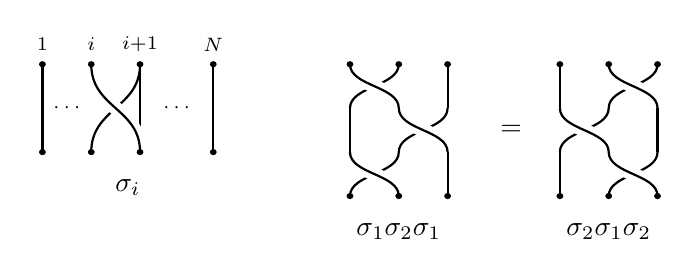
\begin{tikzpicture}[scale=0.62,yscale=0.9]
  % sigma_i on N strands
  \begin{scope}
    \foreach \x in {0,2,3.5} \draw[thick] (\x,0)--(\x,-2);
    \draw[thick] (2,0) .. controls (2,-1) and (1,-1) .. (1,-2);
    \draw[white,line width=5pt] (1,0) .. controls (1,-1) and (2,-1) .. (2,-2);
    \draw[thick] (1,0) .. controls (1,-1) and (2,-1) .. (2,-2);
    \foreach \x in {0,1,2,3.5} {\fill (\x,0) circle (2pt); \fill (\x,-2) circle (2pt);}
    \node[font=\scriptsize] at (0,0.45) {$1$}; \node[font=\scriptsize] at (1,0.45) {$i$};
    \node[font=\scriptsize] at (2,0.45) {$i{+}1$}; \node[font=\scriptsize] at (3.5,0.45) {$N$};
    \node[font=\scriptsize] at (0.5,-1) {$\cdots$}; \node[font=\scriptsize] at (2.75,-1) {$\cdots$};
    \node at (1.75,-2.8) {$\sigma_i$};
  \end{scope}
  % braid relation: left side sigma1 sigma2 sigma1
  \begin{scope}[xshift=6.3cm]
    % level 1: sigma1
    \draw[thick] (1,0) .. controls (1,-0.5) and (0,-0.5) .. (0,-1);
    \draw[white,line width=5pt] (0,0) .. controls (0,-0.5) and (1,-0.5) .. (1,-1);
    \draw[thick] (0,0) .. controls (0,-0.5) and (1,-0.5) .. (1,-1);
    \draw[thick] (2,0)--(2,-1);
    % level 2: sigma2
    \draw[thick] (2,-1) .. controls (2,-1.5) and (1,-1.5) .. (1,-2);
    \draw[white,line width=5pt] (1,-1) .. controls (1,-1.5) and (2,-1.5) .. (2,-2);
    \draw[thick] (1,-1) .. controls (1,-1.5) and (2,-1.5) .. (2,-2);
    \draw[thick] (0,-1)--(0,-2);
    % level 3: sigma1
    \draw[thick] (1,-2) .. controls (1,-2.5) and (0,-2.5) .. (0,-3);
    \draw[white,line width=5pt] (0,-2) .. controls (0,-2.5) and (1,-2.5) .. (1,-3);
    \draw[thick] (0,-2) .. controls (0,-2.5) and (1,-2.5) .. (1,-3);
    \draw[thick] (2,-2)--(2,-3);
    \foreach \x in {0,1,2} {\fill (\x,0) circle (2pt); \fill (\x,-3) circle (2pt);}
    \node at (1,-3.8) {$\sigma_1\sigma_2\sigma_1$};
  \end{scope}
  \node at (9.6,-1.5) {$=$};
  % right side sigma2 sigma1 sigma2
  \begin{scope}[xshift=10.6cm]
    \draw[thick] (2,0) .. controls (2,-0.5) and (1,-0.5) .. (1,-1);
    \draw[white,line width=5pt] (1,0) .. controls (1,-0.5) and (2,-0.5) .. (2,-1);
    \draw[thick] (1,0) .. controls (1,-0.5) and (2,-0.5) .. (2,-1);
    \draw[thick] (0,0)--(0,-1);
    \draw[thick] (1,-1) .. controls (1,-1.5) and (0,-1.5) .. (0,-2);
    \draw[white,line width=5pt] (0,-1) .. controls (0,-1.5) and (1,-1.5) .. (1,-2);
    \draw[thick] (0,-1) .. controls (0,-1.5) and (1,-1.5) .. (1,-2);
    \draw[thick] (2,-1)--(2,-2);
    \draw[thick] (2,-2) .. controls (2,-2.5) and (1,-2.5) .. (1,-3);
    \draw[white,line width=5pt] (1,-2) .. controls (1,-2.5) and (2,-2.5) .. (2,-3);
    \draw[thick] (1,-2) .. controls (1,-2.5) and (2,-2.5) .. (2,-3);
    \draw[thick] (0,-2)--(0,-3);
    \foreach \x in {0,1,2} {\fill (\x,0) circle (2pt); \fill (\x,-3) circle (2pt);}
    \node at (1,-3.8) {$\sigma_2\sigma_1\sigma_2$};
  \end{scope}
\end{tikzpicture}
\caption{Left: the Artin generator $\sigma_i$. Right: the braid relation. In both braids the strand
starting on the left passes over the other two, and the strands starting in the middle and on the right
cross once. The two diagrams differ by sliding the middle crossing past the strand that lies over it.}
\label{TOP:fig:braid}
\end{figure}

The far commutation relation says that exchanges in disjoint regions of the plane can be performed in
either order. This uses the fact that \emph{points take up no room}, a point we return to in
Theorem~\ref{TOP:thm:thick}. A first gem: the braid relation forces all generators to become equal in
the abelianization, and a winding number shows that nothing more collapses, so $B_N$ is infinite.

\begin{proposition}\label{TOP:prop:abel}
For $N\ge2$ the abelianization of $B_N$ is $\Z$, generated by the image of any $\sigma_i$. The
abelianization map is induced by the discriminant
$\Delta(z)=\prod_{i<j}(z_i-z_j)^2\colon\Conf(N,\C)/\Sigma_N\to\C^*$, and it sends every $\sigma_i$ to $1$.
\end{proposition}

\begin{proof}
In an abelian quotient, $\sigma_i\sigma_{i+1}\sigma_i=\sigma_{i+1}\sigma_i\sigma_{i+1}$ becomes
$\sigma_i=\sigma_{i+1}$, so the abelianization is cyclic, generated by $\sigma_1$. Conversely,
$\Delta$ is symmetric, so it is defined on unordered configurations, and it takes values in $\C^*$. Along
$\sigma_i$, the argument of $z_i-z_{i+1}$ changes by $\pi$ while every other factor of $\Delta$ returns to
itself (the factors $(z_i-z_k)$ and $(z_{i+1}-z_k)$ are exchanged), so $\Delta\circ\sigma_i$ winds once around $0$.
Hence $\Delta_*\colon B_N\to\pi_1(\C^*)=\Z$ is onto with $\sigma_i\mapsto1$, and the abelianization is $\Z$.
\end{proof}

\begin{example}[$N=2$]\label{TOP:ex:N2}
$\Conf(2,\C)\cong\C\times\C^*$ via $(z_1,z_2)\mapsto\big(\tfrac{z_1+z_2}2,w=z_1-z_2\big)$, and $\Sigma_2$
acts by $w\mapsto-w$. Squaring identifies $\C^*/\pm1$ with $\C^*$, so
$\Conf(2,\C)/\Sigma_2\cong\C\times\C^*$, $B_2\cong\Z$ generated by $\sigma_1$, and $P_2=2\Z$ generated by the
full twist $\sigma_1^2$ (Figure~\ref{TOP:fig:N2}).
\end{example}

\begin{figure}[ht]
\centering
\begin{tikzpicture}[scale=1.05]
  \begin{scope}
    \draw[->,gray] (-1.6,0)--(1.7,0); \draw[->,gray] (0,-1.4)--(0,1.5);
    \draw[thick,fill=white] (0,0) circle (2pt);
    \fill (1,0) circle (1.6pt) node[below right,font=\scriptsize] {$w$};
    \fill (-1,0) circle (1.6pt) node[below left,font=\scriptsize] {$-w$};
    \draw[addcol,very thick,-{Stealth}] (1,0) arc (0:180:1);
    \node[addcol,font=\scriptsize] at (0.95,1.0) {$\sigma_1$};
    \node[font=\small] at (0,-1.75) {$w=z_1-z_2\in\C^*$};
  \end{scope}
  \draw[-{Stealth},thick] (2.2,0)--(3.4,0) node[midway,above,font=\scriptsize] {$w\mapsto w^2$};
  \begin{scope}[xshift=5.4cm]
    \draw[->,gray] (-1.6,0)--(1.7,0); \draw[->,gray] (0,-1.4)--(0,1.5);
    \draw[thick,fill=white] (0,0) circle (2pt);
    \fill (1,0) circle (1.6pt) node[below right,font=\scriptsize] {$w^2$};
    \draw[addcol,very thick,-{Stealth}] (1,0) arc (0:355:1);
    \node[font=\small] at (0,-1.75) {$\Conf(2,\C)/\Sigma_2\simeq\C^*$};
  \end{scope}
\end{tikzpicture}
\caption{Two points in the plane. The half turn exchanging $z_1$ and $z_2$ is not a loop in
$\Conf(2,\C)$, but it becomes one after the points are unlabelled. Under the identification
$w\mapsto w^2$ it is a generator of $\pi_1(\C^*)$. This is $\sigma_1$, and the discriminant of $(z-z_1)(z-z_2)$ is $w^2$.}
\label{TOP:fig:N2}
\end{figure}

\subsection{Braids from reflection groups}

Now combine Lecture~7 with Lecture~8 and Interlude~A. The space $\Conf(N,\C)$ is the complement in $\C^N$ of the
hyperplanes $z_i=z_j$. These are the \emph{complexified} reflecting hyperplanes of the Weyl group
$W(A_{N-1})=\Sigma_N$. Their real parts cut $\R^N$ into the $N!$ contractible Weyl chambers of Lecture~8. Over $\C$
a hyperplane has real codimension $2$, so the complement is connected, but now loops can wind around the
walls. The Weyl group acts freely on the complement, and
\[
  \pi_1\Big(\big(\C^N\setminus\textstyle\bigcup_{i<j}\{z_i=z_j\}\big)\big/W\Big)=B_N .
\]
The generator $\sigma_i$ is a half turn around the wall $z_i=z_{i+1}$ of the fundamental chamber
$x_1<\dots<x_N$, that is, around the wall of the simple reflection $s_i$. Compare the two presentations:
\[
  W:\ \ s_i^2=1,\ \ (s_is_j)^{m_{ij}}=1;\qquad\qquad
  B_N:\ \ \underbrace{\sigma_i\sigma_j\sigma_i\cdots}_{m_{ij}}=\underbrace{\sigma_j\sigma_i\sigma_j\cdots}_{m_{ij}},
\]
with $m_{ij}=3$ for adjacent nodes of the Dynkin diagram $A_{N-1}$ and $m_{ij}=2$ otherwise. The braid
group is the Coxeter group with the relations $s_i^2=1$ deleted. This works for every diagram of
Lectures~4--5.

\begin{definition}
For a Coxeter matrix $(m_{ij})$, the \emph{Artin group} (or Artin--Tits group) is
$A=\langle\sigma_1,\dots,\sigma_r\mid\underbrace{\sigma_i\sigma_j\sigma_i\cdots}_{m_{ij}}=
\underbrace{\sigma_j\sigma_i\sigma_j\cdots}_{m_{ij}}\ (i\neq j)\rangle$. Adding $\sigma_i^2=1$ recovers the
Coxeter group.
\end{definition}

\begin{theorem}[Brieskorn 1971; Deligne 1972]\label{TOP:thm:BD}
Let $W$ be a finite real reflection group acting on $V=\R^r$, and let $Y_W$ be the complement in $V\otimes\C$
of the complexified reflecting hyperplanes. Then $W$ acts freely on $Y_W$ and $\pi_1(Y_W/W)$ is the Artin
group of the Coxeter diagram of $W$ (Brieskorn). Moreover $Y_W$, and hence $Y_W/W$, is aspherical (Deligne).
\end{theorem}

So every finite Coxeter diagram, including the $E_8$ of the densest packing in dimension $8$, has a braid group. For
$W(B_n)$ the quotient $Y_W/W$ is the space of $n$ unordered points in $\C^*$, and its Artin group is the braid
group of an annulus (Exercise~\ref{TOP:exc:Bn}). For \emph{infinite} Coxeter groups the analogous statement
is the \emph{$K(\pi,1)$ conjecture}, still open in general. For the affine groups, whose fundamental
alcoves appeared in Section~\ref{LIE:sec:torus} as configurations of points on a circle, it was proved by
Paolini and Salvetti (Theorem~\ref{TOP:thm:PS}).

\begin{remark}[Further directions]\leavevmode
\begin{itemize}[nosep]
\item \emph{Linearity.} Braid groups have faithful finite-dimensional representations, by Bigelow and by
  Krammer (Theorem~\ref{TOP:thm:linear}).
\item \emph{Anyons.} For identical quantum particles, exchanges are loops in the \emph{unlabelled}
  configuration space. In $\R^3$ this space has fundamental group $\Sigma_N$, which allows only bosons and fermions. In the plane
  the group is $B_N$, and a one-dimensional representation $\sigma_i\mapsto e^{i\vartheta}$ gives particles with
  any exchange phase. This was observed by Leinaas and Myrheim (Nuovo Cimento, 1977), and Wilczek named the
  particles \emph{anyons} (1982). Non-abelian representations of $B_N$ are the basis of proposals for
  topological quantum computation (Kitaev, 2003; Freedman--Kitaev--Larsen--Wang, Bull.\ AMS, 2003). The
  difference between labelled and unlabelled configurations that we met in Section~\ref{TOP:sec:mintype}
  here has physical consequences.
\end{itemize}
\end{remark}

%======================================================================
\section{Gallery of theorems}
\label{TOP:sec:gallery}

Each statement is followed by a sentence or two on why it belongs in this course.

\subsection*{Min-max and critical points}

\begin{theorem}[Lusternik--Fet 1951; Birkhoff 1917 for $\Sph^2$]
Every closed Riemannian manifold carries a non-constant closed geodesic.
\end{theorem}
\noindent The proof is min-max over a non-trivial homotopy class of maps into the free loop space, which
is the minimax principle of Theorem~\ref{TOP:thm:minimax} in infinite dimensions.

\begin{theorem}[Lusternik--Schnirelmann 1929; Grayson, Ann.\ of Math.\ 1989]
Every Riemannian metric on $\Sph^2$ has at least three simple closed geodesics.
\end{theorem}
\noindent This is the theorem behind Theorem~\ref{TOP:thm:LS}, with $\operatorname{cat}(\R P^2)=3$.
Franks (1992) and Bangert (1993) showed that there are always infinitely many closed geodesics, not
necessarily simple.

\begin{theorem}[Conley--Zehnder, Invent.\ Math.\ 1983]
Every Hamiltonian diffeomorphism of the standard symplectic torus $\T^{2n}$ has at least $2n+1$ fixed points,
and at least $2^{2n}$ if all fixed points are non-degenerate.
\end{theorem}
\noindent This is Arnold's conjecture for tori. The two numbers are exactly
$\operatorname{cat}(\T^{2n})$ and $\sum_\lambda b_\lambda(\T^{2n})$, the degenerate and the Morse counts of
Example~\ref{TOP:ex:torus}.

\begin{theorem}[Marques--Neves, Ann.\ of Math.\ 179 (2014)]\label{TOP:thm:willmore}
Every immersed torus $\Sigma$ in $\R^3$ satisfies
\[
  \mathcal W(\Sigma)=\int_\Sigma H^2\,dA\ \ge\ 2\pi^2,\qquad H=\tfrac12(\kappa_1+\kappa_2).
\]
More precisely, every embedded closed surface of genus $g\ge1$ in $\Sph^3$ has
$\int_\Sigma(1+H^2)\,dA\ge2\pi^2$, with equality if and only if $\Sigma$ is the Clifford torus up to
conformal transformations of $\Sph^3$.
\end{theorem}
\noindent This is the Willmore conjecture (1965). In $\R^3$ the extremal tori are, up to conformal
maps, the torus of revolution with radii in ratio $\sqrt2:1$. The proof is a min-max argument over a
five-parameter family (Section~\ref{TOP:sec:geodesics}).

\begin{theorem}[Marques--Neves, Invent.\ Math.\ 2017; Song, Ann.\ of Math.\ 2023]\label{TOP:thm:yau}
Every closed Riemannian manifold of dimension $3\le n+1\le7$ contains infinitely many smooth, closed,
embedded minimal hypersurfaces. Marques and Neves proved this under the assumption of positive Ricci curvature;
Song proved it in general.
\end{theorem}
\noindent This was conjectured by Yau (1982). The proofs use min-max over families of arbitrarily many
parameters, the analogue of the classes $c_1\le c_2\le\cdots$ in the proof of Theorem~\ref{TOP:thm:LS}.

\subsection*{Configuration spaces of hard particles}

\begin{theorem}[Baryshnikov--Bubenik--Kahle, IMRN 2014]\label{TOP:thm:BBK}
For hard balls of radius $r$ in a rectangular box in $\R^d$ whose shortest side has length $L$, the
critical points of the tautological function are the mechanically balanced configurations. There are no
critical values in $(0,L/2n)$, so $\Conf(n,r)\simeq\Conf(n)$ for $r<L/2n$, and the topology changes just above
$L/2n$.
\end{theorem}
\noindent This is the box version of Theorem~\ref{L10:thm:smalltheta} and of the threshold $2\pi/N$ on the sphere
quoted in Lecture~11. The critical configuration is a row of balls spanning the box, the analogue of
$N$ points equally spaced on a great circle.

\begin{theorem}[Alpert--Kahle--MacPherson, J.\ Appl.\ Comput.\ Topology 5 (2021)]\label{TOP:thm:AKM}
Let $C(n,w)$ be the space of $n$ non-overlapping discs of diameter $1$ in an infinite strip of integer width $w\ge2$, and fix
$j$. If $j\le w-2$, then $H_j(C(n,w))\cong H_j(\Conf(n,\R^2))$ and $b_j$ grows like $n^{2j}$. If $j\ge w-1$,
then $b_j$ grows exponentially in $n$. More precisely, writing $j=q(w-1)+r$ with $0\le r<w-1$,
$b_j\asymp(q+1)^n\,n^{qw+2r}$.
\end{theorem}
\noindent Exponential growth of Betti numbers is a topological counterpart of the exponential count of
jammed states in the channel of Lecture~11, where Fibonacci numbers appeared.

\begin{theorem}[P.~Ramsey, arXiv:2311.16776, 2023]\label{TOP:thm:thick}
For four discs of radius $r$ in the unit disc with $\tfrac14<r\le\tfrac13$, there is a non-trivial
element of $\pi_1$ of the configuration space that becomes trivial when each disc is replaced by its centre.
It is represented by the commutator $\sigma_1^{-1}\sigma_3^{-1}\sigma_1\sigma_3$. For $n\ge5$ discs and
$\tfrac1n<r\le\tfrac1{n-1}$, the configuration space contains a non-contractible $(n-3)$-sphere.
\end{theorem}
\noindent In $B_4$ the relation $\sigma_1\sigma_3=\sigma_3\sigma_1$ makes this commutator trivial. Thick discs have
no room to perform the two exchanges independently, so far commutation \emph{fails} for them. This is a preprint (P.~Ramsey, \emph{Thick braids and other
non-trivial homotopy in configuration spaces of hard discs}).

\begin{theorem}[Farber--Grant, Proc.\ AMS 2009]\label{TOP:thm:farber}
For $n,m\ge2$, $\operatorname{TC}(\Conf(n,\R^m))=2n-1$ if $m$ is odd and $2n-2$ if $m$ is even.
\end{theorem}
\noindent Farber and Yuzvinsky had proved the cases $m=2$ and $m$ odd. The lower bound is a cup-length bound in the spirit of
Theorem~\ref{TOP:thm:cuplength}, using products of ``zero-divisors'' $u\otimes1-1\otimes u$ in
$H^*(\Conf(n,\R^m)\times\Conf(n,\R^m))$.

\subsection*{Braid and Artin groups}

\begin{theorem}[Paolini--Salvetti, Invent.\ Math.\ 224 (2021)]\label{TOP:thm:PS}
The $K(\pi,1)$ conjecture holds for affine Artin groups: for every affine Coxeter group, the quotient of the
complexified complement of the reflection arrangement by the group is a classifying space for the
affine Artin group.
\end{theorem}
\noindent This extends Theorem~\ref{TOP:thm:BD} from the finite Weyl groups of Lectures~4--6 to their affine
versions, whose alcoves are the simplices of Interlude~A.

\begin{theorem}[Bigelow, J.\ AMS 2001; Krammer, Ann.\ of Math.\ 2002]\label{TOP:thm:linear}
The Lawrence--Krammer representation $B_n\to\GL_{n(n-1)/2}\big(\Z[q^{\pm1},t^{\pm1}]\big)$ is faithful for all
$n$. In particular braid groups are linear.
\end{theorem}
\noindent Bigelow's proof is topological: it uses the configuration space of \emph{two} points in the punctured disc.

\subsection*{Rigidity and optimality of packings}

\begin{theorem}[Sch\"utte--van der Waerden, Math.\ Ann.\ 1953; Musin, Ann.\ of Math.\ 2008]
The kissing number is $\kiss_3=12$ and $\kiss_4=24$.
\end{theorem}
\noindent The first settles the Newton--Gregory problem. In the language of these notes it says that
$\max\rho$ on $\Conf(13,\Sph^2)$ is less than $\pi/3$. Musin's proof modifies Delsarte's linear programming method.

\begin{theorem}[Tammes problem: Musin--Tarasov 2012 and 2015; Robinson 1961]
The Tammes problem is solved for $N=13$ (Musin--Tarasov, Discrete Comput.\ Geom.\ 48 (2012); optimal angle
$\approx57.1367^\circ$, unique up to isometry), $N=14$ (Musin--Tarasov, Experiment.\ Math.\ 24 (2015);
$\approx55.6706^\circ$) and $N=24$ (Robinson, Math.\ Ann.\ 1961; the snub cube).
\end{theorem}
\noindent The proofs for $13$ and $14$ enumerate the possible \emph{irreducible contact graphs} by computer.
These are the balanced graphs of Lecture~11, so each proof is the statement that one particular
critical configuration of $\rho$ is the top one. Together with the classical cases ($N\le12$, by Fejes
T\'oth, Sch\"utte--van der Waerden, Danzer and B\"or\"oczky), this covers $N\le14$ and $N=24$.

%======================================================================
\section*{Exercises}
\addcontentsline{toc}{section}{Exercises}

\begin{exercise}
For $f=\sin(\pi x)\sin(\pi y)\sin(\pi(x+y))$ on $\R^2/\Z^2$, show that the index of $\nabla f$ at the origin
is $-2$ (expand $f$ to third order) and check the Poincar\'e--Hopf formula $1+1-2=\chi(\T^2)$. Why can a
function on $\T^2$ with three critical points never be Morse?
\end{exercise}

\begin{exercise}
Using $H^*(\R P^n;\Z/2)=\Z/2[a]/(a^{n+1})$, show that $\operatorname{cat}(\R P^n)\ge n+1$. Deduce that every
smooth function on $\SO(3)\cong\R P^3$, for example a smooth function of the orientation of a rigid
polytope (Lecture~7), has at least four critical points. How many does a Morse function need?
\end{exercise}

\begin{exercise}\label{TOP:exc:N4}
Complete Example~\ref{TOP:ex:N4pass}. (a) Show that if four distinct points lie on a circle in $\Sph^2$, then
two of them are at angular distance at most $\pi/2$, with equality only for a square on a great circle.
(b) Verify the formula for $\rho(u(s))$ and that it is at least $\pi/2$.
\end{exercise}

\begin{exercise}
Compute $P(B\Conf(7))$ and check that the Betti numbers sum to $360$ and that $\chi=24$. If a Morse energy on
$B\Conf(7)$ has $c_0$ local minima, show that it has at least $c_0+13$ critical points of index $1$. (Use the
strong Morse inequality $c_1-c_0\ge b_1-b_0$.)
\end{exercise}

\begin{exercise}
Show that $\Delta=(\sigma_1\sigma_2\sigma_1)^2$ commutes with $\sigma_1$ and $\sigma_2$ in $B_3$, and that it
is the full twist of all three strands. Show that $(\sigma_1\sigma_2)^3=\Delta$. Under the abelianization of
Proposition~\ref{TOP:prop:abel}, what is the image of $\Delta$?
\end{exercise}

\begin{exercise}\label{TOP:exc:Bn}
The Weyl group $W(B_n)=(\Z/2)^n\rtimes\Sigma_n$ has reflecting hyperplanes $x_i=\pm x_j$ and $x_i=0$. Show
that the map $(z_1,\dots,z_n)\mapsto\{z_1^2,\dots,z_n^2\}$ identifies $Y_{W(B_n)}/W(B_n)$ with the space of
$n$ unordered distinct points in $\C^*$. Write down the Artin relations for the diagram $B_n$, with
$m=4$ on the double edge, and interpret the extra generator as a strand going around the puncture.
\end{exercise}

\begin{exercise}\label{TOP:exc:TC}
(a) Show that $\operatorname{TC}(X)=1$ if and only if $X$ is contractible. (b) Show that
$\operatorname{TC}(\Sph^1)=2$ by writing down two explicit motion planners. (c) Two robots move
without collision on a circular track. Identify the configuration space and compute its $\operatorname{TC}$.
\end{exercise}

\begin{exercise}
Show that $C(n,1)$, the space of $n$ discs of diameter $1$ in a strip of width $1$, has exactly $n!$ connected
components and that each is contractible. Compare with $\Conf(n,\R)$ in Lecture~7. (This is the case
$w=1$, excluded from Theorem~\ref{TOP:thm:AKM}; Alpert, Kahle and MacPherson record $b_0=n!$ and $b_j=0$
for $j\ge1$.)
\end{exercise}

\section*{Further reading}
\addcontentsline{toc}{section}{Further reading}
\begin{itemize}[nosep]
\item J.~Milnor, \emph{Morse Theory}, Annals of Math.\ Studies 51, 1963. Part~I is the basis of
  Lectures~8--10 and of Lemma~\ref{TOP:lem:deform}.
\item O.~Cornea, G.~Lupton, J.~Oprea, D.~Tanr\'e, \emph{Lusternik--Schnirelmann Category}, AMS Math.\ Surveys and
  Monographs 103, 2003. Category, cup-length, and critical point theory.
\item M.~Struwe, \emph{Variational Methods}, Springer. Min-max and the mountain pass in infinite dimensions.
\item F.~C.~Marques, A.~Neves, \emph{The Willmore conjecture}, arXiv:1409.7664. A survey of the proof.
\item Y.~Baryshnikov, P.~Bubenik, M.~Kahle, \emph{Min-type Morse theory for configuration spaces of hard
  spheres}, Int.\ Math.\ Res.\ Not.\ 2014(9), 2577--2592.
\item C.~Kassel, V.~Turaev, \emph{Braid Groups}, Springer GTM 247, 2008.
\item M.~Farber, \emph{Invitation to Topological Robotics}, EMS Zurich Lectures in Advanced Mathematics, 2008.
\item R.~Ghrist, \emph{Elementary Applied Topology}, 2014. Configuration spaces, robots, and Morse theory
  for applications.
\end{itemize}
